\hypertarget{kiemelt-fejlesztesi-teruletek}{%
\section{Kiemelt fejlesztési
területek}\label{kiemelt-fejlesztesi-teruletek}}

A tantárgyak a Budapest Schoolban a tanulás tartalmának minimumát
jelölik ki, a tantárgyi struktúrát a Nemzeti alaptanterv határozza meg.
Az iskola a tantárgyakon átívelő fejlesztési területeket határoz meg.
Szeretnénk, hogy a gyerekek folyamatosan fejlődjenek a világ tudományos
megismerésében (STEM), a saját és mások kulturális közegéhez való
kapcsolódásban (KULT), valamint a testi-lelki egyensúlyuk fenntartásában
(Harmónia).

Az iskolában egy foglalkozás egyszerre több fejlesztési irányelvnek is
megfelelhet. Egy modul során gépesíthetünk egy ökológiai
tangazdaságot (STEM) úgy, hogy közben megismerjük a gazdálkodás történelmi
és szocio-kulturális hátterét (KULT), és a szabad levegőn végzett
munkával a testünket és a lelkünket egyaránt ápoljuk (Harmónia).

\hypertarget{termeszet--es-mernoki-tudomany-technologia-es-matematika-stem}{%
\subsection{Természet- és mérnöki tudomány, technológia és\\ matematika
(STEM)}\label{termeszet--es-mernoki-tudomany-technologia-es-matematika-stem}}

A STEM ma már nem csak néhány tantárgy összevonása és mozaikszóban való
emlegetése miatt releváns. Az interdiszciplináris tudós-mérnöki
szemlélet, a fejlesztő-kutató munka, az innováció az élet minden
területén megjelenik, és nem csak eldugott laborok mérnökeinek a
feladata új dolgokat felfedezni, kipróbálni, alkotni. Ezt az is mutatja,
hogy a világ legnagyobb mértékben bővülő munkáinak több mint fele
STEM-alapú, és ezek száma a következő évtizedekben a kutatások szerint
nőni fog. A STEM a jövő nagy kérdéseit hivatott megválaszolni. Épp ezért
a STEM a felfedezés és a megismerés iránti vágyat kell, hogy ébren
tartsa és tovább mélyítse a gyerekekben, miközben gyakorlatias alkotó
módszerével fejleszti a csapatmunkát és a kitartást, valamint azt, hogy
a megszerzett ismereteket új, korábban nem tapasztalt helyzetekben is
alkalmazni tudják. Ez az a szemléletmód, ami egyaránt segítheti az egyén
akadémiai tudásának fejlődését és a tanulás iránti hosszú távú
elköteleződését.

\begin{figure}
\centering
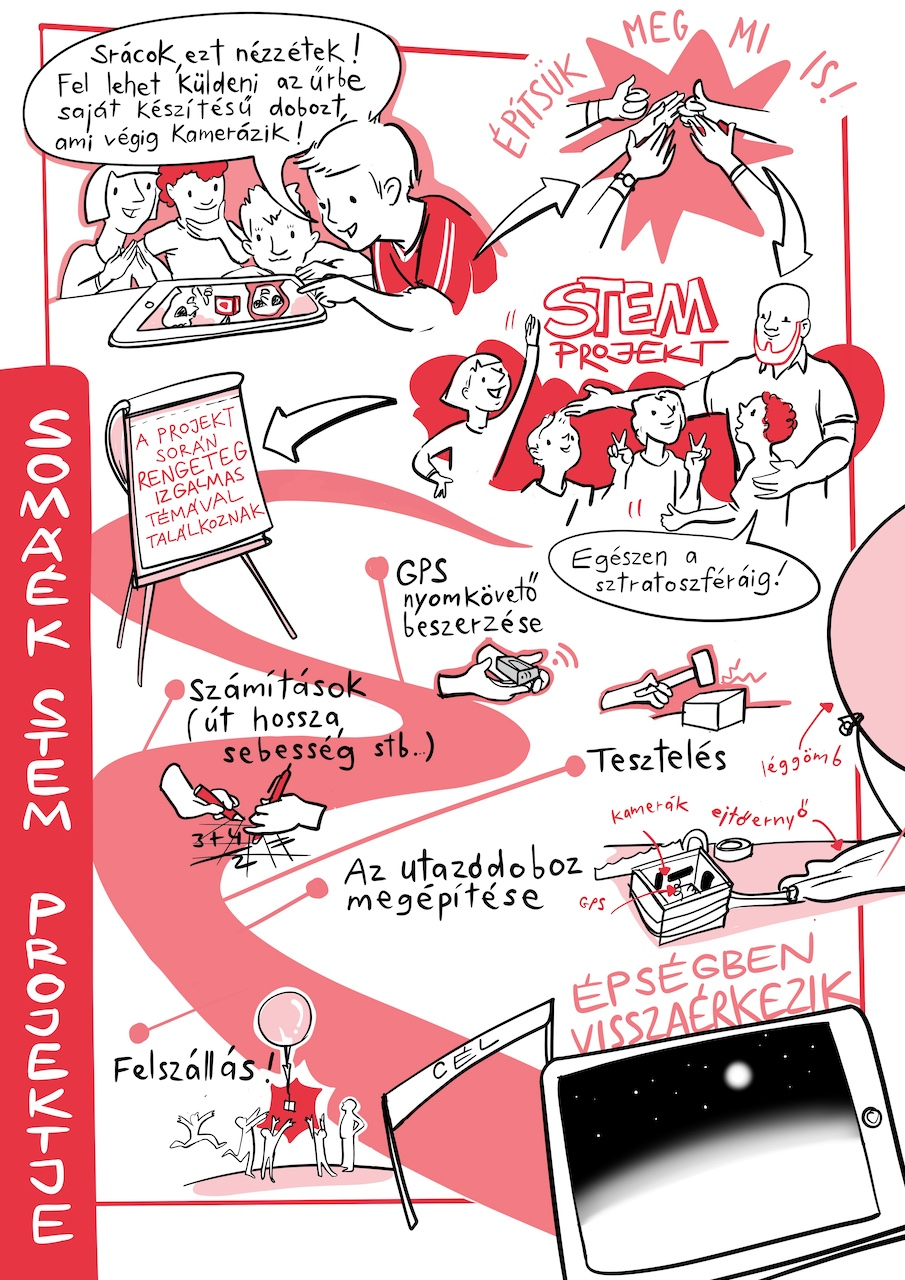
\includegraphics{pics/2a_stem.jpg}
\caption{A STEM a felfedezés és megismerés vágyát tartja ébren.}
\end{figure}

\hypertarget{stem-fejlesztesi-celok}{%
\paragraph{STEM fejlesztési célok}\label{stem-fejlesztesi-celok}}

\begin{itemize}
\item
  Problémamegoldási képesség fejlesztése
\item
  Matematikai gondolkodás fejlesztése
\item
  Logikus gondolkodás fejlesztése
\item
  A világ működésének mélyebb megértése a természettudományos
  szemléleten keresztül
\item
  Innovatív fejlesztésekhez szükséges technológiai (kódolás) és
  gyakorlati (maker) eszköztár megismerése és alkalmazása
\end{itemize}

A STEM komplex, tudományterületeken és a technológiai lehetőségeken
átívelő megközelítése sokfelé ágazik, mégis vannak olyan alapszabályai,
amelyek a tanulás során mindig jellemzik. Ahhoz, hogy folyamatos
fejlődés legyen, fontos, hogy a tanulás az aktuális képességekhez igazodó,
nyitott, tényeken alapuló, kutatásalapú, diverz módszertanú,
skálázható legyen,
és releváns módon történjen a STEM területen.

A STEM terület a fenti célok eléréséhez a következő egymást segítő
komponensek alkalmazását javasolja:

\hypertarget{gyakorlatias-tanulas-elkotelezett-es-egyuttmukodo-kozossegek-halozatahoz-kapcsolodva}{%
\paragraph{Gyakorlatias tanulás elkötelezett és együttműködő közösségek
hálózatához
kapcsolódva}\label{gyakorlatias-tanulas-elkotelezett-es-egyuttmukodo-kozossegek-halozatahoz-kapcsolodva}}

A STEM-tanulás során különösen fontos, hogy az adott területet jól
ismerő szaktanár és a mentoron túl további innovatív és segítő közegek
is támogassák a gyerekek fejlődését. Sokat hozzátehet a mindennapi
élethez való kapcsolódás kialakításában, ha intézményi (pl. múzeum,
kutatóintézet) vagy technológiai, ipari és más STEM-hez kapcsolódó
területen működő cégeknél dolgozó emberek mintákat mutatnak, vagy akár
bekapcsolódnak a gyerekek mindennapos munkájába.

\hypertarget{hozzaferheto-tanulasi-gyakorlatok-amelyek-a-jatek-es-a-kockaztatas-eszkozeit-is-felhasznaljak}{%
\paragraph{Hozzáférhető tanulási gyakorlatok, amelyek a játék és a
kockáztatás eszközeit is
felhasználják}\label{hozzaferheto-tanulasi-gyakorlatok-amelyek-a-jatek-es-a-kockaztatas-eszkozeit-is-felhasznaljak}}

A STEM tematikájú játékok segítik a gyerekeket abban, hogy egymástól és
együtt is tanuljanak, ezzel fejlesztik a kreativitásukat és a felfedezés
iránti vágyukat. Ezek a felfedeztető játékok ráirányítják a fókuszt a
csapatmunka fontosságára, és arra, hogy miként lehet mai problémákra és
kihívásokra válaszokat találni.

\hypertarget{multidiszciplinaris-tanulasi-elmenyek-amelyek-a-vilag-nagy-kihivasaira-keresnek-valaszokat}{%
\paragraph{Multidiszciplináris tanulási élmények, amelyek a világ nagy
kihívásaira keresnek
válaszokat}\label{multidiszciplinaris-tanulasi-elmenyek-amelyek-a-vilag-nagy-kihivasaira-keresnek-valaszokat}}

A STEM legfőbb kihívása, hogy a mai kor olyan kérdésfelvetéseit
vizsgálja, amelyekre közösségi, nemzeti vagy globális\break
szinten még
nincsenek meg a válaszok. Ezek lehetnek a vízgazdálkodással, az
agykutatással és annak a prevencióra, vagy épp a gyógyulásra gyakorolt
hatásaival, a megújuló energiagazdálkodással, vagy épp az önvezető autók
új generációjának technológiai irányaival kapcsolatosak.

Ezek a kihívások egyúttal azt is megmutatják, hogy mely kérdések
lehetnek a kultúránk szempontjából relevánsak.

\hypertarget{rugalmas-es-nyitott-tanulasi-kornyezet}{%
\paragraph{Rugalmas és nyitott tanulási
környezet}\label{rugalmas-es-nyitott-tanulasi-kornyezet}}

A STEM élményszerű tanulásához nagyban hozzájárulhatnak a nyitottan
értelmezett tanulási környezetek. Az iskolai terek alkotótérré
változtatásával, a természeti közegekben végzett terepmunkák vagy a
korszerű technológiai platformok, mint például a VR (virtuális valóság
-- virtual reality) vagy AR (kiterjesztett virtuális valóság --
augmented virtual reality) bevonásával a területek könnyebben
megismerhetővé válnak, és újabb kérdések feltevésére sarkallhatják a
gyerekeket, miközben az irányító tanárszerep helyett a kísérletező,
segítő és facilitátor feladatok erősödnek.

\hypertarget{a-tanulasi-eredmenyek-meresenek-uj-eszkoztara}{%
\paragraph{A tanulási eredmények mérésének új
eszköztára}\label{a-tanulasi-eredmenyek-meresenek-uj-eszkoztara}}

A teljesítmény, a kutatás, a kísérletezés és az alkotás kiemelt fókuszú
a gyerekek STEM tanulási útja során. Kiemelt szerepet kapnak ezért a
saját kutatásokra épülő prezentációk, megfigyelések és az azokra adott
értékes visszajelzések.

\hypertarget{kultura-tarsadalom-kommunikacio-es-muveszetek-kult}{%
\subsection{Kultúra, társadalom, kommunikáció és művészetek
(KULT)}\label{kultura-tarsadalom-kommunikacio-es-muveszetek-kult}}

A művészetek és önmagunk kifejezése az őskortól segítik az embereket a
túlélésben. A képzelet absztrakciós szintjének alkalmazása az egyik
legfontosabb faji tulajdonsága az embernek. Ennek fejlesztése pedig
globális világunk egyik legnagyobb kihívása. Ahhoz, hogy a társadalmi
viták és szabályozások aktív alakítójává válhassunk, hogy megismerjük a
globális világunk legnagyobb kihívásait, értenünk kell a múltunkat, a
saját kultúránkat és a kultúrák szerepét általában, és ki kell tudnunk
fejezni magunkat olykor szavakkal, máskor a művészet eszközeivel.

Még soha nem élt az emberiség ennyire behálózott világban, és még soha
nem kellett ennyire tudatosan készülnünk arra, hogy gyerekeinknek
többféle kultúrát, társadalmi hálózatot kell megérteniük, és abban
eligazodniuk. Családok, munkahelyi és lakókörnyezeteink, sőt még a
nemzeti és az azokat átívelő társadalmi környezetek is gyorsabban
változnak ma, mint szüleink életében. Ezért szeretnénk, hogy gyerekeink
stabil identitásukra építkezve képesek legyenek emberként emberekhez
kapcsolódni, embertársaikat megérteni, velük együtt élni, dolgozni.

\begin{figure}
\centering
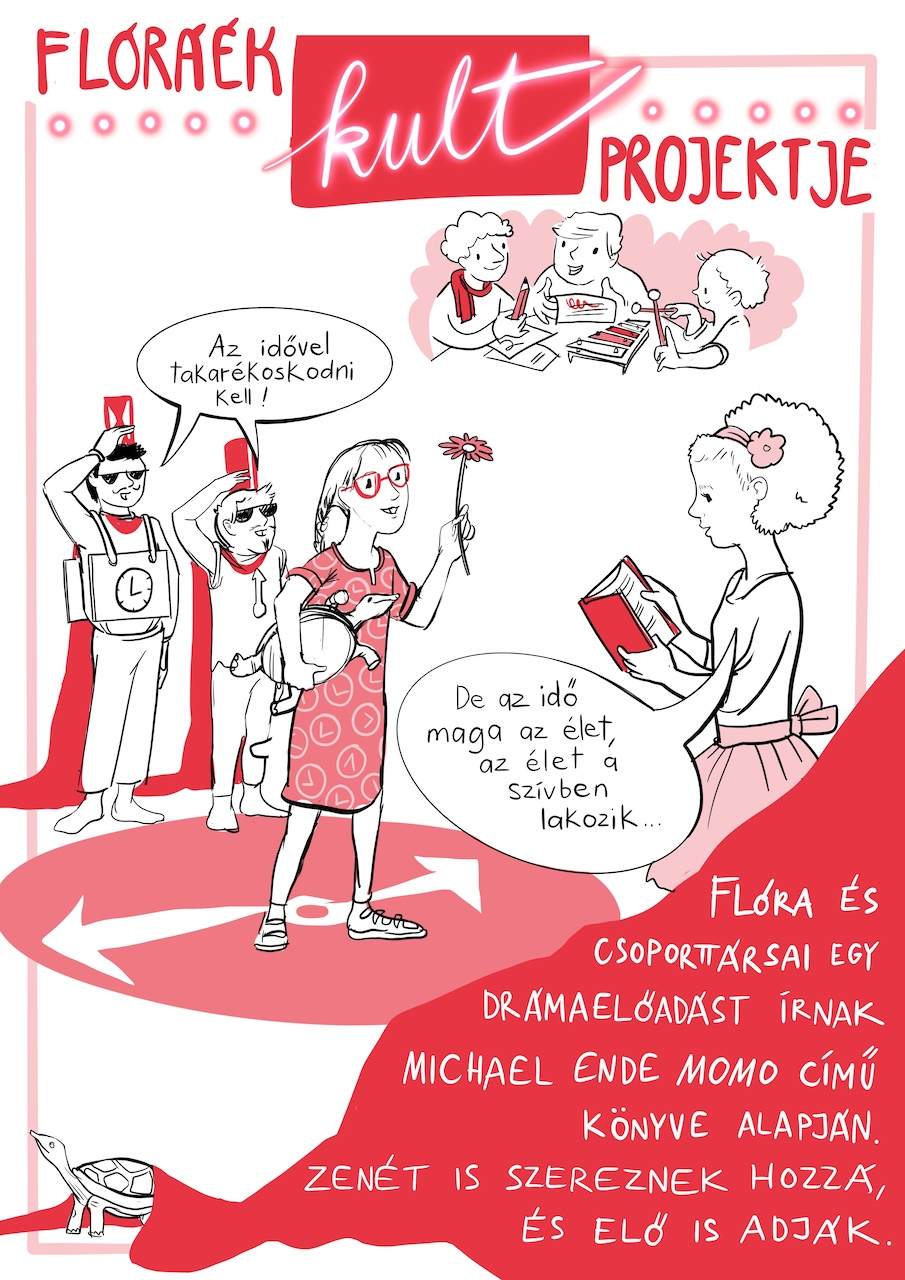
\includegraphics{pics/2b_kult.jpg}
\caption{A tanulóközösség egy családias közösség.}
\end{figure}

A tanulás egyik legfőbb funkciója, hogy képessé váljunk egy fenntartható
élet kialakítására. Ehhez pedig önmagunk, környezetünk (Harmónia) és a
világ működésének megismerésén (STEM) és fejlesztésén túl a szűk és
tágabb értelemben vett kulturális tereinkhez is kapcsolódnunk kell
(KULT). Meg kell ismernünk a lokális és a globális kihívásokat ahhoz,
hogy értő, empatikus módon kapcsolódhassunk a saját és más kultúrákhoz,
és a fenntartható fejlődés alakítójává válhassunk. A Budapest \mbox{School}
KULT terület fő célja ezért az olyan globális kompetenciák fejlesztése,
amelyek a fenti cél elérését támogatják.

A KULT terület a következő fejlesztési területeket foglalja magába:

\begin{itemize}
\item
  írott és beszélt anyanyelvi kommunikáció
\item
  írott és beszélt idegen nyelvi kommunikáció
\item
  mai lokális és globális kihívások megismerése a múlt kontextusában
\item
  kulturális diverzitás és a kultúra mint az emberi viselkedést leíró
  eszköztár megismerése
\item
  művészetek stílus- és formavilága
\item
  művészetek mint önkifejezési eszköz a vizuális (hagyományos
  képzőművészetektől a digitális művészetekig) és előadóművészetekben
  (dráma, tánc, zene)
\end{itemize}

Miközben világunkban egyre nő a technológia szerepe, folyamatosan nő az
igény arra is, hogy képesek legyünk értelmezni és megfelelően használni
az elénk táruló információt. Ennek alapja a megfelelő szövegértés, a
nyelvnek mint írott és verbális kommunikációs stratégiának az egyéni és
korosztályi képességekhez mért alkalmazása, valamint a művészeteken
keresztül a kifejezés egyéb módjainak elsajátítása. Ahhoz, hogy képessé
váljunk erre, megfelelő történelmi és kulturális kontextusba kell
helyeznünk az elénk táruló információt, és nyitottnak kell lennünk arra,
hogy ezeket befogadjuk, és a mai kor globális kihívásaihoz képest
értelmezhessük.

A KULT komplex tanulási struktúrája adja meg az új információk
elmélyülésének alapjait, és segít abban, hogy a mindennapos döntési
stratégiáink részévé váljanak.

A KULT az alábbi képességeket fejleszti:

\begin{itemize}
\tightlist
\item
  Empátia és együttérzés
\item
  Egyéni és közösségi hiedelmek felismerése
\item
  Mérlegelő gondolkodás
\item
  A művészetek és az irodalom funkciójának felismerése és a mindennapi
  életbe való beépítése
\item
  Az etika és a morál alapkérdéseinek felfedezése és megkérdőjelezése
\item
  Új ötletek befogadása
\item
  Az emberiség kulturális örökségének és aktuális diverzitásának
  kiaknázása
\item
  Többsíkú gondolkodás, multidiszciplináris szövegértés
\end{itemize}

A KULT terület a fenti célok eléréséhez a következő egymást segítő
komponensek alkalmazását javasolja:

\hypertarget{helyi-kozossegekhez-valo-kapcsolodas}{%
\paragraph{Helyi közösségekhez való
kapcsolódás}\label{helyi-kozossegekhez-valo-kapcsolodas}}

Tanulás során a lokális közösségek szerepe megnő, hiszen mind a saját
kultúra és művészeti értékek megismerése, mind a nyelvhasználat
tekintetében döntő szerepe van annak, hogy saját környezetünkben tudjuk
ezeket érteni és alkalmazni.

\hypertarget{kortars-kihivasok}{%
\paragraph{Kortárs kihívások}\label{kortars-kihivasok}}

A KULT alapját a kortárs művészeti értékek, a kortárs problémák és
kihívások adják. Ezek ugyan mindig a múlt és a környezet kontextusában
értelmezhetők, de elsődleges módszer a kapcsolat kialakítása a mai világ
alkotásaival, szövegeivel, kulturális értékeivel.

A KULT abban segít a gyerekeknek, hogy jobban eligazodjanak a mai és
holnapi világban, és olyan kérdéseket tegyenek fel, amelyek ma még
megválaszolatlanok, és a jövőt formálhatják. Ehhez a művészetek, nyelvek
és kultúrák találkozási pontjait, az átmeneteket is célszerű szemlélni.

\hypertarget{rugalmas-es-befogado-tanulasi-kornyezet}{%
\paragraph{Rugalmas és befogadó tanulási
környezet}\label{rugalmas-es-befogado-tanulasi-kornyezet}}

A mai szövegek értelmezése, az online elérhető tartalmakban való
tájékozódás képessége éppoly fontos, mint az idegen nyelveken történő
kommunikáció elősegítése a világhoz történő kapcsolódással. Az aktuális
globális kihívásokat a múltunkon keresztül érthetjük meg, amihez
tanulási környezetünket folyamatosan a megismerés igényeihez képest kell
formálnunk, és olyan eszközöket kell használnunk, amelyek az értelmezést
segíthetik.

\hypertarget{alkotoi-szabadsag-es-az-alkoto-szabad-ertelmezese}{%
\paragraph{Alkotói szabadság és az alkotó szabad
értelmezése}\label{alkotoi-szabadsag-es-az-alkoto-szabad-ertelmezese}}

Az önálló alkotói munka és az alkotások szabad értelmezése és befogadása
az innováció és a kreativitás alapja. Ennek biztosításához a hagyományos
keretek újraértelmezésére van szükség és arra, hogy egy alkotói
folyamatban a saját cél kibontakozásának támogatása megtörténjen.

\hypertarget{harmonia-fizikai-lelki-jollet-es-kapcsolodas-a-kornyezethez}{%
\subsection{Harmónia (fizikai, lelki jóllét és kapcsolódás a
környezethez)}\label{harmonia-fizikai-lelki-jollet-es-kapcsolodas-a-kornyezethez}}

Testi és lelki egészségünk az alapja annak, hogy tanulhassunk,
fejlődhessünk, és a saját életünk alakítóivá váljunk. Életünk fizikai,
lelki, érzelmi és társas aspektusai határozzák meg a kapcsolódásunkat
önmagunkhoz, társainkhoz és az őket körülvevő emberekhez, vagyis a
tágabb értelemben vett társadalomhoz. Ez segít abban, hogy önálló
döntéseket hozzunk, és jól tudjunk együtt tanulni, dolgozni
csoportokban. Ahhoz, hogy a közösségünk részeként harmóniában élhessünk
önmagunkkal, az épített és természeti környezetünkhöz is kapcsolódnunk
kell.

A Budapest School tanulási koncepciójának középpontjában az egyén, mint
a közösség jól funkcionáló, saját célokkal rendelkező tagja áll. Az
iskolában való fejlődése során elsősorban azt tanulja, hogy miként tud
specifikált saját célokat megfogalmazni, és hogyan tudja ezeket elérni.
Ebben a folyamatban egy mentor segíti a munkáját az iskola kezdetétől a
végéig. Ő figyel arra, hogy a gyerek fizikai és lelki biztonsága és
fejlődése folyamatos legyen, és segíti azokban a helyzetekben, amikor
biztonságérzete vagy stabilitása csökken.

A közösségben jól funkcionáló egyén belső harmóniájához a következő
fejlesztési területeket tartja az iskola fontosnak:

\begin{itemize}
\item
  Érzelmi és társas intelligencia
\item
  Önismeret és önbizalom
\item
  Konfliktuskezelés
\item
  A nehéz élethelyzetekkel történő megküzdés készségei (reziliencia)
\item
  Mérlegelő gondolkodás
\item
  Közösségi szabályok alkotásában való részvétel és azok alkalmazása
\item
  Csapatmunka gyakorlati fejlesztése
\item
  Oldott játék
\item
  Egészséges testi fejlődés
\item
  Saját igényekhez képest megfelelő táplálkozás
\item
  A természettel való kapcsolódás
\item
  Épített falusi és városi környezetben való eligazodás
\item
  A technológia világában felhasználói szintű eligazodás és annak\break
  harmonikus alkalmazása
\end{itemize}

A Harmónia a fenti célok eléréséhez a következő egymást segítő
komponensek alkalmazását javasolja:

\hypertarget{kozossegben-csapatban}{%
\paragraph{Közösségben, csapatban}\label{kozossegben-csapatban}}

A Budapest School egy közösségi iskola, ahol a közösség tagjai egymással
és egymástól tanulnak. A közösségekhez való tartozáshoz, a csapatban
való gondolkodáshoz, és a családban való működéshez szükséges
képességeket leginkább úgy tudjuk fejleszteni, ha azt a kezdetektől
megéljük. A közösség belső szabályainak megalkotása és az azokhoz való
kapcsolódás a tanulás folyamatosságának alapfeltétele.

\hypertarget{eletkepessegek-life-skills}{%
\paragraph{Életképességek (life
skills)}\label{eletkepessegek-life-skills}}

Szeretnénk, ha gyerekeink általában alkalmazkodóan (adaptívan) és
pozitívan tudnának hozzáállni az élet kihívásaihoz, ha lelki és fizikai
erősségük és ellenálló képességük (rezilienciájuk) megmaradna és
fejlődne. A Egészségügyi Világszervezet {\autocite{WHO1999}} a
következőképpen definiálta az életképességeket:

\begin{itemize}
\item
  Döntéshozás, problémamegoldás
\item
  Kreatív gondolkodás
\item
  Kommunikáció és interperszonális képességek
\item
  Önismeret, empátia
\item
  Magabiztosság (asszertivitás) és higgadtság
\item
  Terhelhetőség és érzelmek kezelése, stressztűrés
\end{itemize}

\hypertarget{erzelmi-intelligencia}{%
\paragraph{Érzelmi intelligencia}\label{erzelmi-intelligencia}}

Sokszor kiemeljük az érzelmi intelligenciát, hangsúlyozva, hogy
gyerekeinknek többet kell foglalkozniuk az érzelmek felismerésével,
kontrollálásával és kifejezésével, mint szüleiknek kellett.

\hypertarget{szabad-mozgas-es-seta}{%
\paragraph{Szabad mozgás és séta}\label{szabad-mozgas-es-seta}}

A különböző mozgásformák, a sportok és a séta mindennapivá tétele
természetes módon, a gyerekek saját igényei szerint kell, hogy történjen.

\hypertarget{gyakorlatias-mindennapi-kepessegek}{%
\paragraph{Gyakorlatias, mindennapi
képességek}\label{gyakorlatias-mindennapi-kepessegek}}

Ahhoz, hogy gyerekeink önállóan és hatékonyan tudják élni életüket, hogy
a társakhoz való kapcsolódás ne függőség legyen, egy csomó praktikus
mindennapi tudást el kell sajátítaniuk. A gyerekeknek folyamatosan
fejleszteniük kell az élethez szükséges mindennapi tudást a
levélszemét-kezeléstől az internet és a szociális média tudatos
használatán át egészen a személyi költségvetés elkészítéséig.

\hypertarget{egeszseges-taplalkozas}{%
\paragraph{Egészséges táplálkozás}\label{egeszseges-taplalkozas}}

Az egészséges táplálkozás tanulható viselkedésforma, melynek alapja
nemcsak a megfelelő élelmiszerek kiválasztása, hanem azok élettani
hatásainak megismerése és az étkezési szokások alakítása is.
